\documentclass{article}
% Language setting
% Replace `english' with e.g. `spanish' to change the document language
\usepackage[swedish]{babel}

% Set page size and margins
% Replace `letterpaper' with`a4paper' for UK/EU standard size
\usepackage[a4paper,top=2cm,bottom=2cm,left=3cm,right=3cm,marginparwidth=1.75cm]{geometry}

% Useful packages
\usepackage{amsmath}
\usepackage{graphicx}
\usepackage{cite}
\usepackage[colorlinks=true, allcolors=blue]{hyperref}
\usepackage[square,numbers]{natbib}

\title{Helmholtzspole \\ Att bestämma elektronens massa}
\author{Linus Lind}

\begin{document}
\maketitle
%\section{Introduktion}
Denna laboration syftar till att bestämma massen hos elektronen. Med hjälp av en Helmholtzspole bestäms elektronens massa $m_e = 8,93 \times 10^{−31} \pm 0,84 \times10^{−31}$.

\section*{Teori}
Magnetfältet för Helmholtzspole, se fig \ref{fig:coil} för illustration av utrustning, är approximativt homogent. Flödestätheten i mitten av spolen \cite{anderson1999design}
\begin{equation}
    B_H = \frac{\gamma_0 N I_s}{R}
\end{equation}
där $R$ är spolens radie, $N$ antal varv, $I_s$ strömmen genom spolen. Från permabiliteten i vakum, $\mu_0$, bestäms   
\begin{equation}
\gamma_0 = \left( \frac{4}{5} \right)^{3/2} \mu_0  \approx 8.99 \times 10^{-7} \: \mathrm{N/A^2}    
\end{equation}.
I Uppställningen, se fig \ref{fig:coil}, accelereras elektroner med spänning $U_{acc}$ till hastighet $v$ . Under antagande att magnetfältet är homogent  kommer elektronerna inta en cirkulär bana i med radie $r$ i magnetfältet. Det är den magnetiska kraften som utgör den centralaccelererande kraften för cirkelrörelsen. Banradien uppfyller således
\begin{equation}
Q_e v B_H = \frac{ m_e v^2}{r}
\end{equation}
där $Q_e$ är elektronens laddning. 
 
\section*{Metod}
\begin{figure}
    \centering
    \begin{subfigure}
        \centering
        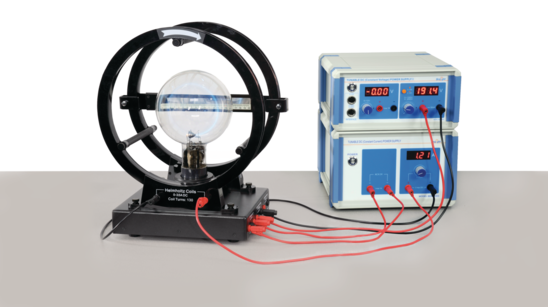
\includegraphics[height=1.5in]{helmsetup.png}
    \end{subfigure}
    \begin{subfigure}
        \centering
        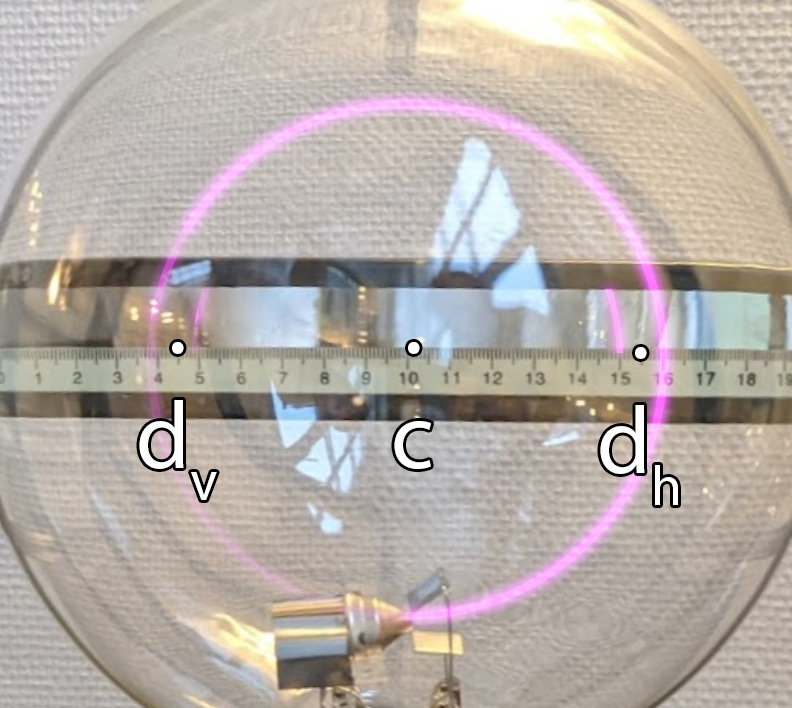
\includegraphics[height=1.5in]{helmbeam.png}
    \end{subfigure}
    \caption{\label{fig:coil}Till vänster den experimentella uppställningen med Helmholtzspole i dagsljus. Till höger ett visualisering av elektronstrålen med markeringar för elektronbanans centrum $C$, tillsammans den vänstra position $d_v$ och den högra $d_h$. Parallax förskjutningen av banan mot dess spegelbild är tydlig för både $d_v$ och $d_h$. }
\end{figure}
Med en given ström och accelerationsspänning genomförs mätning av banradien i tre steg
\begin{enumerate}
  \item linjalen centreras i så att mätsidan går igenom mitten av den cirkulära banan, $C$ i fig \ref{fig:coil}. Betraktningsvinkel är viktig. Värdet avläses då centrum för elektronbanan och dess spegelbild sammanfaller. 
  \item Med hjälp av spegelbilden av den cirkulära banan bestäms det positionen av cirkelns vänstra position $d_v$, se fig \ref{fig:coil}. För noggran avläsning är betraktningsvinkel viktigt. Avläsning görs då vänstra delen av elektronbanan, dess spegelbild och $d_v$ alla överlappar. I fig \ref{fig:coil} skulle detta åstadkommas genom att skifta betraktningsvinkeln mer åt vänster.
  \item Analog avläses det högra positionen $d_h$.
\end{enumerate}
Ur differensen av $d_h$ och $d_v$ fås elektronbanans diameter vilket ger radien.

\begin{table}[h]
\centering
\caption{\label{tab:results} $d_v$, $d_h$, $U_{acc}$ och $I_s$ utgör mätvärdena. Med (1)-(3) bestäms $B_H$ och $m_e$ ur mätvärdena. \\}
\begin{tabular}{c|c|c|c|c|c|c}
$d_v$ (cm)& $d_h$ (cm) & $r$ (m)& $U_{acc}$ (V)& $I_s$ (A)& $B_H$ (T)& $m_e$ (kg)\\ \hline
7,2 & 12,5 & 0,027 & 120,2 & 2,00 & 1,44×10^{-3} & 9,69×10^{-31}\\
4,9 & 15,0 & 0,051 & 125,0 & 1,00 & 7,19×10^{-4} & 8,46×10^{-31}\\
5,0 & 13,8 & 0,044 & 143,6 & 1,28 & 9,21×10^{-4} & 9,16×10^{-31}\\
4,0 & 15,1 & 0,056 & 150,0 & 1,00 & 7,19×10^{-4} & 8,51×10^{-31}\\
4,0 & 14,0 & 0,050 & 170,0 & 1,20 & 8,63×10^{-4} & 8,78×10^{-31}\\
3,6 & 14,3 & 0,054 & 176,9 & 1,16 & 8,34×10^{-4} & 9,02×10^{-31}\\
4,4 & 13,0 & 0,043 & 194,0 & 1,50 & 1,08×10^{-3} & 8,89×10^{-31}
\end{tabular}
\end{table}
\section*{Resultat}
För sju stycken slumpvis valda spolströmmar $Is$ och accelerationsspänningar $U_{acc}$ avläses cirkelbanans vänstra och högra position, $d_v$ respektive $d_h$. Utifrån dessa mätvärden och (1)-(3) bestäms flödestätheten $B_H$ och elektronmassan $m_e$. Se tabell \ref{tab:results} för sammanställning. Ur resultat bestäms ett 95\% konfidensintervall för elektron massan till $m_e = 8,93 \times 10^{−31} \pm 0,84 \times10^{−31} $.



\begin{figure}[h]
\centering
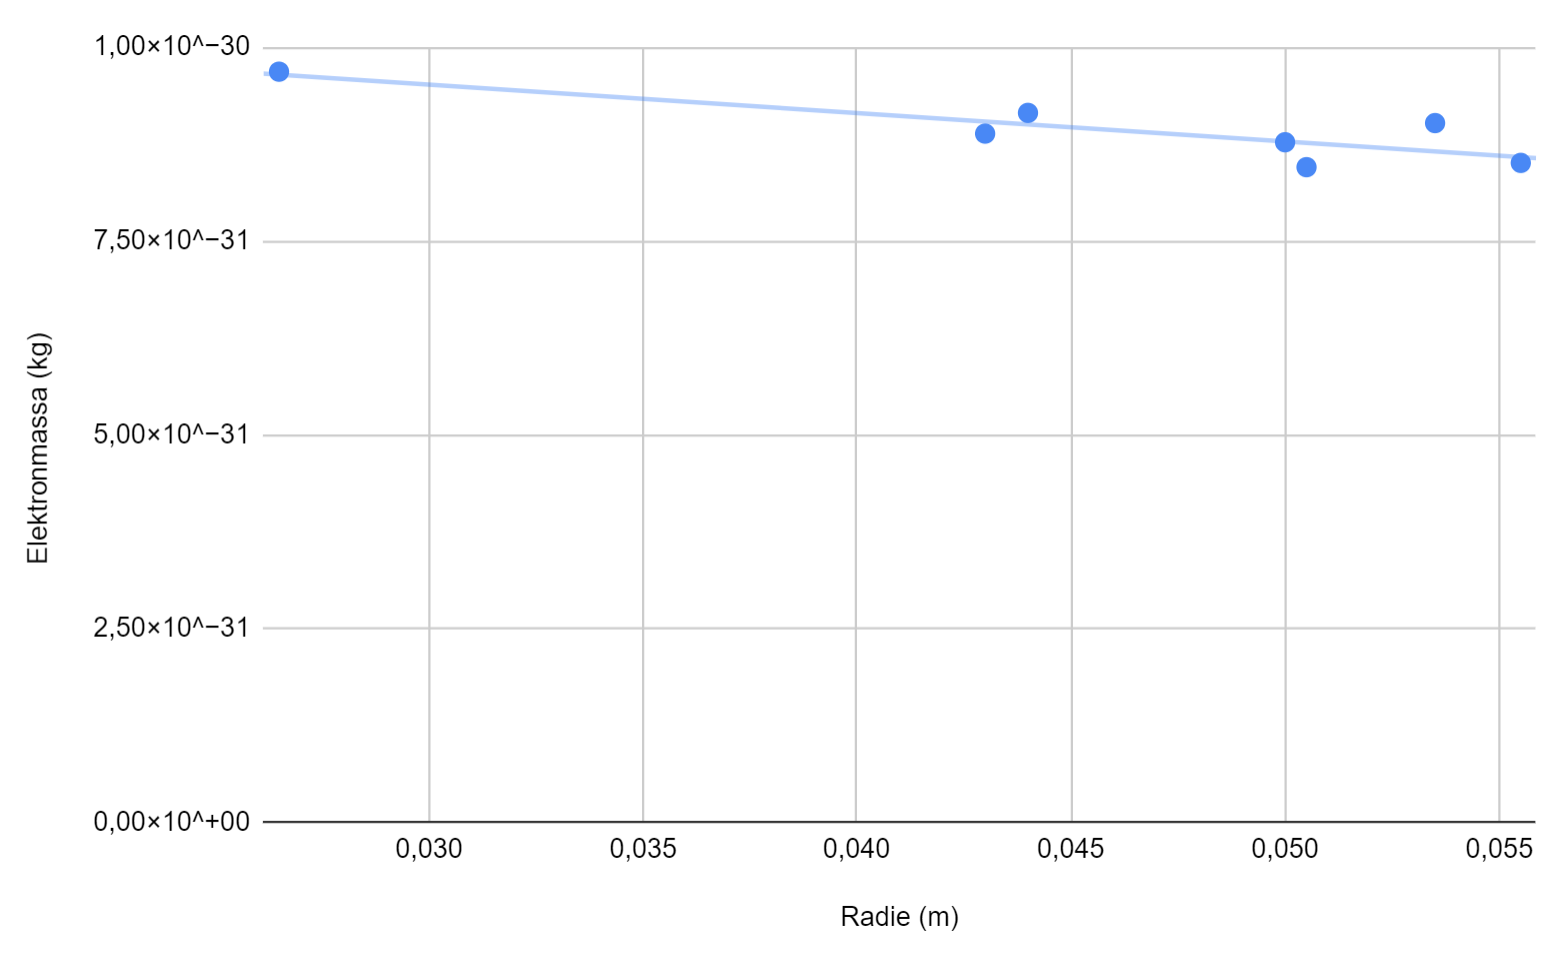
\includegraphics[width=0.5\textwidth]{trendmass.png}
\caption{\label{fig:masstrend}Den beräknade elektron massan som funktion av strålradie.}
\end{figure}

\section*{Diskussion}
Tidigare resultat för elektronens massa är $m_e=9,1147\times 10^{-31} \pm 0,00133\times10^{-31}$ \cite{cohen1952rydberg} vilket ligger inom felmarginalerna från resultatet ovan.

De utmaningen i utförandet var avläsningen av det högra och vänstra värdet, $d_v$ och $d_h$. Elektronsstrålens är utbredd och suddig vilket gör det svårt att avläsa positionen noggrant. Vidare är det svårt att att positioner ögat så att cirkelns periferi , dess spegelbild och mätvärdet på linjalen alla är på en linje. Speciellt då dessa kräver att laborant fokuserar på olika djup. Potentiellt skulle båda dessa problem kunna kunna avhjälpas genom att fota positionen för att där efter genomföra en mer noggran bedömning, med mindre variation mellan mätningar. 

Magnetfältet från Helmholtzspolen uppfyller (1) i centrum av spolen\cite{anderson1999design}. En bättre förståelse för hur magnetfältet varierar i spolen skulle kunna bidra till att $U_{acc}$ och $I_s$ väljs så att $r$ befinner sig i ett område område där (1) är representativt för den faktiska magnetiska flödestätheten. I fig \ref{fig:masstrend} kan vi se hur det finns en viss trend att det beräknade elektronmassan varierar systematisk med radie på elektronbanan. Denna variation skulle kunna tillskrivas att magnetfältet varierar i Helmholtzspole en vidare undersökning, med syfte att bygga en bättre förståelse för eventuella varianser i flödestätheten, behövs att kunna tolka resultatet.

\newpage
\bibliographystyle{abbrvnat}
\bibliography{sample}

\end{document}